\documentclass[conference]{IEEEtran}
\IEEEoverridecommandlockouts
% The preceding line is only needed to identify funding in the first footnote. If that is unneeded, please comment it out.
%----------------------------------------------------------
\usepackage{cite}
\usepackage[pdftex]{graphicx}
% declare the path(s) where your graphic files are
\graphicspath{images/}
\DeclareGraphicsExtensions{.pdf,.jpeg,.png,.jpg}
\usepackage{amsmath,amssymb,amsfonts}
\usepackage{algorithmic}
\usepackage{graphicx}
\usepackage{textcomp}
\usepackage{array}
%\usepackage[caption=false,font=normalsize,labelfont=sf,textfon =sf]{subfig}
\usepackage{dblfloatfix}
\usepackage{url}
\usepackage{lipsum}
\usepackage{listings}
\usepackage{xcolor}
\def\BibTeX{{\rm B\kern-.05em{\sc i\kern-.025em b}\kern-.08em
    T\kern-.1667em\lower.7ex\hbox{E}\kern-.125emX}}
%----------------------------------------------------------
    \lstset{
        escapeinside={/*@}{@*/},
        language=Python,	
        basicstyle=\fontsize{8.5}{12}\selectfont,
        numbers=left,
        numbersep=2pt,    
        xleftmargin=2pt,
        frame=tb,
        columns=fullflexible,
        showstringspaces=false, 
        tabsize=4,
        keepspaces=true,
        showtabs=false,
        showspaces=false,
        morekeywords={inline,public,class,private,protected,struct},
        captionpos=b,
        lineskip=-0.4em,
        aboveskip=10pt,
        extendedchars=true,
        breaklines=true,
        prebreak = \raisebox{0ex}[0ex][0ex]{\ensuremath{\hookleftarrow}},
        keywordstyle=\color[rgb]{0,0,1},
        commentstyle=\color[rgb]{0.133,0.545,0.133},
        stringstyle=\color[rgb]{0.627,0.126,0.941},
    }
%----------------------------------------------------------

\begin{document}

\title{Jogo Pong - aplicações de Aruino e Processing 4\\
{\footnotesize \textsuperscript{*} Sistemas Embarcados: Prof. Marco Reis - marco.reis@ba.docente.senai.br}
\thanks{Identify applicable funding agency here. If none, delete this.}
}

% \author{\IEEEauthorblockN{Marco Reis, 41650-010\IEEEauthorrefmark{1}}
% \IEEEauthorblockA{\IEEEauthorrefmark{1}Robotics & Autonomous Systems Center,
% Senai Cimatec, Salvador, Brazil}% <-this % stops an unwanted space


\author{\IEEEauthorblockN{1\textsuperscript{st} Rodrigo Freire Bastos}
\IEEEauthorblockA{\textit{Engenharia Elétrica} \\
\textit{Senai Cimatec}\\
Salvador, Brasil \\
rodrigo.bastos@aln.senaicimatec.edu.br}
\and
\IEEEauthorblockN{2\textsuperscript{nd} Akin Silva}
\IEEEauthorblockA{\textit{Engenharia Elétrica} \\
\textit{Senai Cimatec}\\
Salvador, Brasil \\
akin.silva@aln.senaicimatec.edu.br}

}


\maketitle

\begin{abstract}
 O trabalho desenvolvido é um sistema embarcado para o jogo eletônico pong com baixo custo, feito usando
 processing como interface gráfia e um arduino com dois potenciometros como 
 controles para o jogo.
\end{abstract}

\begin{IEEEkeywords}
Sistema embarcado, Pong, Arduino, Processing.
\end{IEEEkeywords}

\section{Introdução}

O jogo Pong é um jogo eletrônico do genero Arcade desenvolvido
em 1972 pela Atari, Inc. O jogo consiste no conceito de ping pong
introduzido numa versão 2D. 

\begin{figure}[htbp]
    \centerline{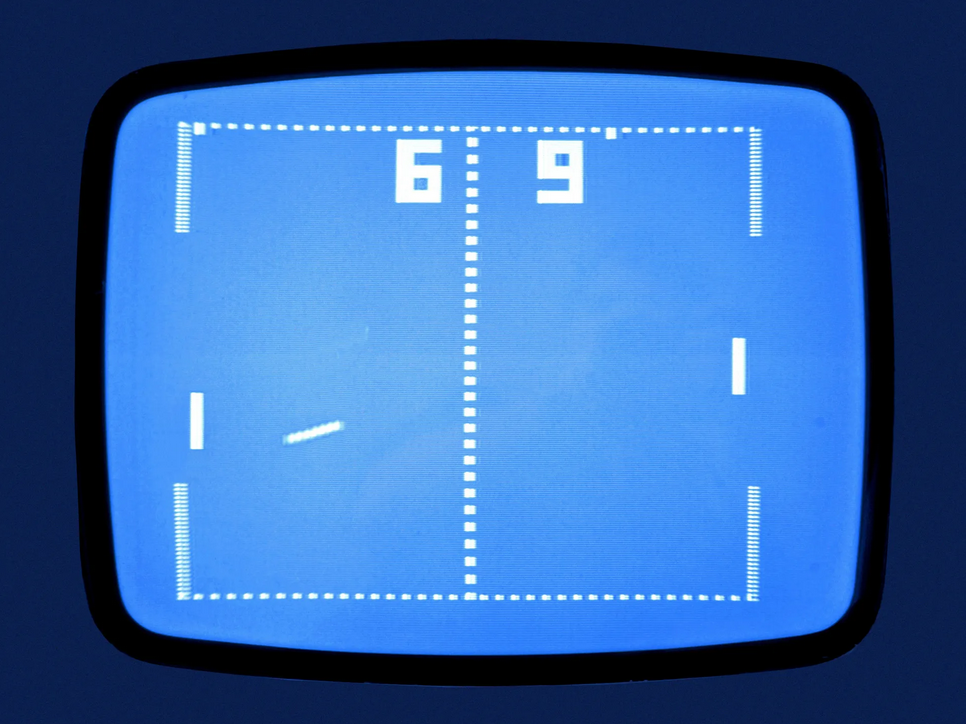
\includegraphics[width=0.4\textwidth]{/home/rod/Desafio_03/images/Screenshot from 2022-07-03 02-55-52.png}}
    \caption{Pong game}
    \label{fig}
    \end{figure}


Dessa maneira, o jogo para duas pessoas PvP ou PvIA tem como objetivo
rebater a bola afim de fazer-la passar ultrapassar a barra do adversário
e no fim, quem fizer mais ponto vence [2].

\subsection{Processing}
Processing é um software open Source e linguagem de programação
com base em java que utiliza artificios gráficos para representar
artes visuais. Hoje, o processing possui uma enorme comunidade que 
ajuda a desenvolver diversos programas de niveis educaionais a profissonais [3].


\subsection{Arduino}
Arduino é uma plataforma de prototipagem, é um software open Source que abrage
toda a área da microeletrônica e microcontroladores. Hoje o desenvovimento em arduinos pode 
ser realizado pela própria plataforma de arduino, a Arduino IDE, que possui todo suporte
para o arduino e suas placas. Além do mais, o arduino possui uma vasta comunidade muito ativa 
e que fornece um grande suporte aos iniciantes, tornando essa plataforma num ótimo começo
na eletrônica [1].



\section*{Desenvolvimento}

\subsection{Objetivo geral}
O objetivo desse desafio é montar um sistema embarcado refazendo o clássico jogo Pong, usando arduino e processing.

\subsection{Objetivo específico}
    \begin{itemize}
    \item Montar o arduino com 2 potenciometros e 2 pushbuttons;
    \item montar o código do pong no processing; 
    \item Montar uma conexão serial entre o arduino e o processing;
    \item mover as barras do pong com os potenciômetros;
    \item 2 pushbuttons para ralizar a função start e reset do jogo.
    \end{itemize}
 
\section{Materiais}
 \begin{itemize}
     \item arduino UNO R3;
     \item dois(2) potenciômetros de $ 1K\Omega $;
     \item dois(2) pushbuttons;
     \item dois(2) Resistores de $ 127\Omega $;
     \item Cabos para conexão;
     \item Placa de ensaio.
 \end{itemize}

\subsection{Métodos}
A construção do desafio foi dividida em duas partes, hardware e software. 

A construção do hardware começou com o cabeamento do sensor ultrassônico, que possui 4 portas: VCC e GND (para
energizar o sensor) e Trigger e Echo (para enviar e receber dados de distâncias, respectivamente). Da mesma maneira,
foi conectado um LED rgb que possui 4 portas: red (vermelho), green (verde), blue (azul) e GND. Além do display LCD (16x2)
que para conexão, são 16 pinos, dos quais usamos 12 para uma conexão básica, já incluindo as conexões de alimentação (pinos 1 e 2),
 backlight (pinos 15 e 16) e contraste (pino 3).

 \begin{figure}[htbp]
    \centerline{\includegraphics[width=0.4\textwidth]{/home/rod/Pictures/Screenshots/Screenshot from 2022-05-25 22-05-10.png}}
    \caption{Sensor ultrassônico (HC-SR04)}
    \label{fig}
    \end{figure}

    \begin{figure}[htbp]
        \centerline{\includegraphics[width=0.2\textwidth]{/home/rod/Pictures/Screenshots/Screenshot from 2022-05-25 22-00-02.jpg}}
        \caption{LED RGB}
        \label{fig}
        \end{figure}

        \begin{figure}[htbp]
            \centerline{\includegraphics[width=0.4\textwidth]{/home/rod/Pictures/Screenshots/Screenshot from 2022-05-25 22-07-15.png}}
            \caption{LCD (16x2)}
            \label{fig}
            \end{figure}


\section{Metodologia}
 A atividade desenvolvida foi realizada com conhecimentos prévios sobre C++ e eletrônica básica em Arduinos, porém, para sanar as dúvidas e dificuldades encontradas no
 desenvolvimento da atividade foram utilizadas documentações de bibliotecas no site (1), e para realizar todo experimento foi utilizada a plataforma Tinkercad, que é
 muito bem otimizada além de ser gratuita e ser capaz de realizar simulações.

\section{Resultados}
 Ao concluir as conexões e códigos percebeu-se que só era possível ler e imprimir a informação passada de um arduino para outro caso houvesse um delay de ao menos 3 segundos
 entre cada envio de informação, dessa maneira o sistema não ficou muito otimizado, visto que, são necessários ao menos 3 segundos para executar sua função, e, por conta
 do delay do sistema a LED RGB também ficou com um certo delay para mudar de cor. Por outro lado, o sistema desenvolvido consegue ler corretamente as distâncias em cm 
 , identificar em qual região ela pertence e por consequência alertar a proximidade do objeto de com uma LED RGB inserida no sistema e também informar a disância do objeto
 em um LCD conectado no segundo arduino por meio de uma conexão serial.

\section*{Referências}

\begin{enumerate}
    \item Arduino. Arduino, 2022. Disponível em: www.arduino.cc. Acesso em: 25/maio/2022;
    \item Britannica, The Editors of Encyclopaedia. "Pong". Encyclopedia Britannica, Invalid Date, https://www.britannica.com/topic/Pong. Accessed 3 July 2022.
    \item Processing. Processing.org. Disponível em: https://processing.org/. Acesso em: 03/07/2022.
\end{enumerate}

\end{document}
